\begin{figure}[h]
\centering
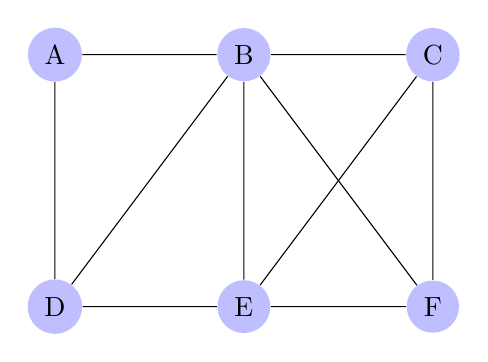
\begin{tikzpicture}
[scale=.8,auto=left,every node/.style={circle,fill=blue!25}]
  \node (n6) at (3,2) {D};
  \node (n4) at (3,6) {A};
  \node (n5) at (6,2) {E};
  \node (n1) at (6,6) {B};
  \node (n2) at (9,2) {F};
  \node (n3) at (9,6) {C};
  \foreach \from/\to in {n6/n4,n4/n1,n6/n1,n6/n5,n1/n3,n1/n2,n1/n5,n5/n2,n5/n3,n3/n2}
    \draw (\from) -- (\to);
\end{tikzpicture}
\caption{Hamiltionvej og Hamiltionkreds} 
\label{hamiltion_vej_kreds}
\end{figure}